\documentclass[11pt,a4paper]{article}
\usepackage[utf8]{inputenc}
\usepackage[english]{babel}
\usepackage{amsmath}
\usepackage{amsfonts}
\usepackage{amssymb}
\usepackage{graphicx,float}
\usepackage{subcaption}
\usepackage{float}
\begin{document}
	\author{\textbf{Yaren Aksel}}
	\title{\textbf{Experiment 2, Applications of Lasers}}
	\date{November 22, 2019}
	\maketitle
	\textit{with} {\large\textit{{Onuray Sancar}}\textit{,} \textit{Experiment Date}: November 15, 2019\\[2\baselineskip]
		\textbf{Abstract}\\[\baselineskip]
		\par The purpose of the experiment is to observe preciseness of lasers when making measurements. We have calculated a distance by using an old method named triangulation and our value is $3\sigma$ away from the measured value. We have measured the wavelength of our laser by using gratin and we have found the values as $\lambda=(5.5\pm3.7)\times100$nm which is 0.22$\sigma$ away from the given value. We have measured the diameter of a hair and the value we have found is in the range of human hair. Finally, we have measured the index of refraction of a transparent solid by using Michelson's interferometer and the value we have is $n=1.09\pm0.14$.
		\\[\baselineskip]
		\textbf{Theoretical Motivation}
		\\[\baselineskip]
		\par Lasers are devices that emit narrow beams of intense electromagnetic radiation(light). A laser beam has the special property that the light waves emitted are all in step with one another and usually of one wavelength, or color. Without understanding quantum theory profoundly, the laser wouldn't be developed because the roots of the laser go back Einstein. He proposed that light is composed of tiny packets of wave energy, photons. Also, he theorised that if an excess energy is given to atoms of a material, they will emit photons and then these photons could stimulate nearby atoms to emit further photons. All the photons would have the same energy and wavelength and move off in the same direction. 
		\par After 40 years of Einstein's proposition, this idea converted into a practical laser by Theodore Maiman and his team.$^{[1]}$
		\par The Michelson interferometer is a widely used device. As we know LIGO detected gravitational waves with this kind of device. It is used for making precise measurements and is
		based on the interference of light. The device uses a beam splitter to split the incident beam along two different paths, and then recombine them. The two beams recombine to produce an interference pattern. If the optical path length changes along either of the two arms then the interference pattern changes. Constructive interference occurs when the path difference is an integral number of wavelengths.
		\par The trianglation is a very old method. Since the basics of trigonometry was extablished in ancient times, the distances were measured using this technique. In our experiment we have used laser for measuring a distance.
		\begin{figure}[H]
			\begin{center}
				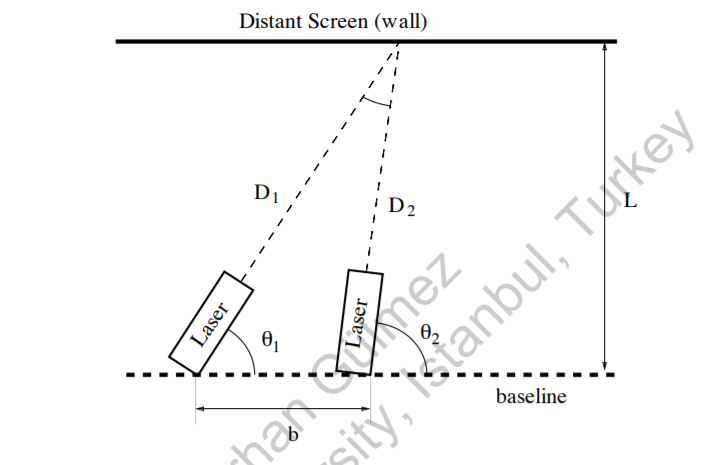
\includegraphics[scale=0.6]{triang.png}
			\end{center}
		\end{figure}
		As we see from the figure the laser is placed two different location and making two different angle with the baseline and at these two different situations it is projected to the same point. Let's derive an equation to find L.
		\begin{equation}
		D_2.sin\theta_2=D_1.sin\theta_1=L
		\end{equation}
		\begin{equation}
		D_2.cos(\theta_2)+b=D_1.cos\theta_1
		\end{equation}
		Then inserting $D_2=D_1.sin\theta_1/sin\theta_2$ to equation(1)
		\begin{equation}
		b=D_1(cos\theta_1.sin\theta_2-sin\theta_1cos(\theta_2))/sin\theta_2
		\end{equation}
		\begin{equation}
		D_1=b\times sin\theta_2/sin(\theta_2-\theta_1)=b\times sin(\pi-\theta_2)/sin(\theta_2-\theta_1)
		\end{equation}
		Inserting this to the equation(1)
		\begin{equation}
		D_2=b\times sin\theta_1/sin(\theta_2-\theta_1)
		\end{equation}
		By just inserting this to the equation(1) we can determine L.
		\par For the second part of the experiment we should mention about reflecting grating. A reflecting grating with widely speced grooves gives good diffraction spectra if the incedent light is nearly parallel to the surface of the grating. Let's derive the formula for wavelength.
		\begin{figure}[H]
			\begin{center}
				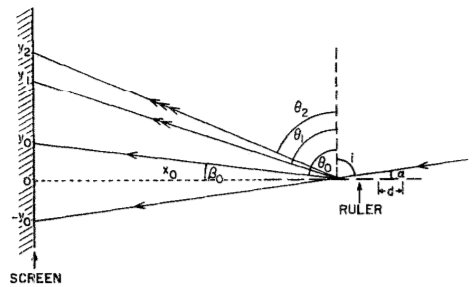
\includegraphics[scale=0.7]{cetvel.png}
			\end{center}
		\end{figure}
	    As we see from the figure we can write the grating equation as
	    \begin{equation}
	    n\lambda=d(sini-sin\theta)
	    \end{equation}
	    where n is an integer, $\lambda$ is the wavelength, and d is the spacing between rulings. It is more convenient to write $\alpha=90^o-i, \beta=90^o-\theta$ then the equation becomes
	    \begin{equation}
	    n\lambda=d(cos\alpha-cos\beta)
	    \end{equation}
	    Also, $\alpha=\beta_0$ and $tan\beta=y_n/x_0$ because $\beta$ is small, so that $tan\beta\approx sin\beta$.$^{[2]}$
	    	\begin{figure}[H]
	    	\begin{center}
	    		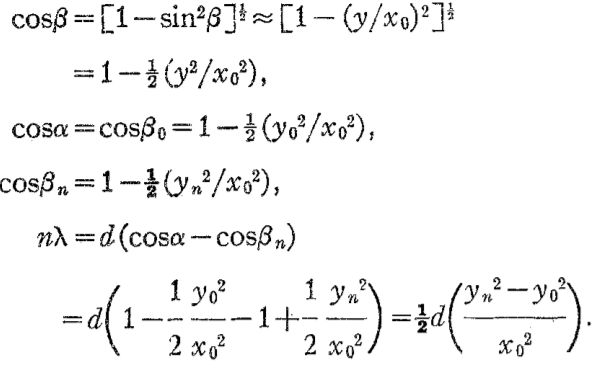
\includegraphics[scale=0.7]{cet.png}
	    	\end{center}
	    \end{figure}
    \par For the third part of the experiment: When light passes through a single slit whose width w is on the order of the wavelength of the light, then we can observe a single slit diffraction pattern on a screen that is a distance L >> w away from the slit.  The intensity is a function of angle.  Huygens' principle tells us that each part of the slit can be thought of as an emitter of waves.  All these waves interfere to produce the diffraction pattern.  Where crest meets crest we have constructive interference and where crest meets trough we have destructive interference.$^{[3]}$
    By using the one slit equation $dsin\theta_n=n.\lambda$ where n=1,2,3,... we can calculate the diameter of hair d by looking at angles from the horizontal line where the hair is placed. Here, molecular distance of hair's molecules is so small compared to the diameter of the hair. Therefore, we can neglect the these molecular distances because their effect on the diffraction pattern is negligible.
    \par For the fourth part of the experiment: index of refraction a material decribes how fast light travels through the material. When light enters to a material there will be phase difference compared to the light travelling the same distance in the air. Using these phase differences we can easily determine index of refraction. The optical path differences can be measured very accurately with the help of a Michelson's interferometer.$^{[4]}$
    \par Assume that we have a transparent solid object whose thickness is d and its index of refraction is n. For normal incidence of light rays, the optical path length is
    \begin{equation}
    L_{perpendicular}=n.d+\frac{d}{cos\theta_i}-d
    \end{equation}
		Let's rotate the sample around its vertical axis by an angle of $\theta$ and also the light incident on the sample is falling on the surface at and angle of $\theta$ with the normal to the surface of the sample.
			\begin{figure}[H]
			\begin{center}
				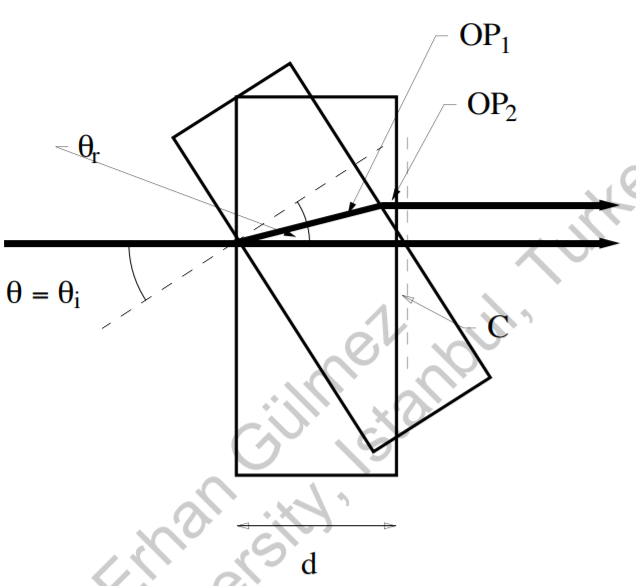
\includegraphics[scale=0.6]{n.png}
			\end{center}
		\end{figure}
	    We can determine the angle of refraction inside the solid from the Snell's law($n_{air}=1$)
	    \begin{equation}
	    \frac{sin\theta_i}{sin\theta_r}=n.
	    \end{equation}
	    If we didn't rotated the sample and again we send the light perpendicular to the sample's axis then, $L_{perpendicular}=n.d+\frac{d}{cos0}-d$=nd. Therefore, for the rotated case by using simple geometry 
	    \begin{equation}
	    OP_1=\frac{nd}{cos\theta_r}
	    \end{equation}
	    Then to find $OP_2$ we first project $OP_1$ to the horizontal line which is $OP_1\times cos(\theta_i-\theta_r)$. Then, we should substract this result from nd
	    \begin{equation}
	    OP_2=nd-\frac {nd}{cos\theta_r}cos(\theta_i-\theta_r)=
	    \end{equation}
	    \begin{equation}
	    OP_2=\frac{d}{cos\theta_r}sin(\theta_i-\theta_r)tan(\theta_i)
	    \end{equation}
	    Then, the total optical path length when the transparent solid sample is at an angle $\theta$ with respect to the incident beam is
	    \begin{equation}
	    L_{theta}=OP_1+OP_2=\frac {nd}{cos\theta_r}(1+\frac {sin(\theta_i-\theta_r)tan\theta_i}{n}).
	    \end{equation}
	    Then, the net difference in the optical path length between rotated and unrotated cases is
	    \begin{equation}
	    \Delta L= L_{\theta}- L_{perpendicular}	
	    \end{equation}
	    In the Michelson interferometer, rotating the sample slowly will shift the interference pattern. The number m of fringes shifted will be 
	    \begin{equation}
	    m=\frac {2\Delta L}{\lambda}
	    \end{equation}
	    Then, tying to pull n in the equation to the left of the equation. We get
	    \begin{equation}
	    n=\frac {(d-m\lambda/2)(1-cos\theta_i)}{d(1-cos\theta_i)-m\lambda/2}
	    \end{equation}
	    \\[\baselineskip]
	    Error propagation
	    \begin{equation}
	    {\sigma }_{f}=\sqrt{\sum _{i}^{n}{\left(\frac{\partial f}{\partial {x}_{i}}\right)}^{2}{\sigma }_{{x}_{i}}^{2}+\dots }
	    \end{equation}
		Weighted average
		\begin{equation}
		f_{weighted}=\frac{\sum _{i}\frac{{f}_{i}}{{\sigma_i }^{2}}}{\sum _{i}\frac{1}{{\sigma_i }^{2}}}
		\end{equation}
		where $\sigma_i$ is the uncertainty in $f_i$\\[\baselineskip]
		\textbf{Apparatus, Experimental Procedure, Data}
\\[\baselineskip] \textbf{\small{Apparatus}}(mainly)
\begin{itemize}
	\item \textbf{Low Power He-Ne Laser}: It is main apparatus of the experiment. It is used for observing optical phenomena.
	\item \textbf{Ruler}: It is used for measuring distances.
	\item \textbf{Protractor}: It is used for measuring angle that the laser make with the base line.
	\item \textbf{Metal Ruler}: It is used as grading.
	\item \textbf{Hair}: It is used to observe the phenomenon of one slit diffraction.
	\item \textbf{Michelson's Interferometer}: It is used to determine index of refraction of a solid sample from path difference.
	\item \textbf{A Transparent Solid Sample}: By sending laser beam to it we determined its index of refraction.
\end{itemize}
\textbf{\small{Procedure}}
\begin{enumerate}
	\item First, we closed the lights in the room to observe patterns of the laser properly.
	\item For the first part of the experiment we drew a line on the table parallel to the wall. Then we placed the laser as making angle 80$^o$ with the base line and we marked the wall where the laser beam projected. After that we rotated the laser as making angle 73$^o$ with the baseline and as it projects on the same point we marked. Then we measured the distance between the first place and the second place of the laser.
	\item In the second part of the experiment we tried to observe diffraction pattern of the laser on the wall. For this we placed a ruler on the table and we ascended the laser and projected the laser from its ascending position to the ruler. We have seen the diffraction pattern on the wall. Then we measured the positions of the maximas.
	\item In the third part of the experiment we have tried to determine diameter of a hair. To do that we projected the laser beam on the hair and then we saw the diffraction pattern on the wall. Then, we measured the positions of the minimas and the distance between hair and the wall.
	\item In the fourth part of the experiment we tried to determine index of refraction of a transparent solid sample by using Michelson's interferometer. We first tried to observe how we get the most clear image on the wall. Then we placed the solid sample in one of the arms of Michelson's interferometer perpendicular to the light beam. After that we rotated the sample holder slowly while counting the number of fringes appearing.
\end{enumerate}
\textbf{\small{Data}}\\[\baselineskip]
\par The first part of the experiment:
\begin{figure}[H]
	\begin{center}
		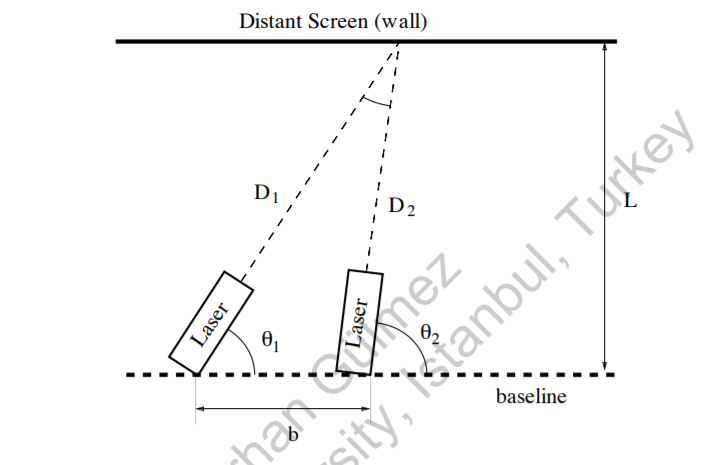
\includegraphics[scale=0.7]{t.png}
	\end{center}
\end{figure}
\par b=$13.80\pm0.05$cm, $L=104.2\pm0.1cm$, $\theta_1=73\pm1^o$ and $\theta_2=80\pm1^o$.
The second part of the experiment:
\begin{center}
	\begin{figure} [H] 
		\begin{tabular}{|c |c|} \hline
			$y_n$& Height of the patterns from the ruler's placed axis(cm) \\ [0.5ex] 
			\hline
			$y_0$&3.8 \\
			\hline
			$y_1$ & 6.7\\
			\hline 
			$y_2$ &8.8\\
			\hline 
			$y_3$& 10.5 \\
			\hline 
			$y_4$& 12.0\\
			\hline 
			$y_5$&13.4\\
			\hline 
			$y_6$& 14.7\\
			\hline
			$y_7$&15.9\\
			\hline		
		\end{tabular}
		\caption{The distance between the wall and the ruler is $L=121.3\pm0.8$cm, spacing between the ruler is d=0.05cm and it is taken as given. Errors of the $y_n$s's are 0.1cm. The accepted value of the wavelength of the laser is 633nm.}
	\end{figure}
\end{center}
The third part of the experiment:
\begin{center}
	\begin{figure} [H] 
		\advance\leftskip-1.50cm
		\begin{tabular}{|c |c||c| c|} \hline
			$y_n$& Vertical distances of patterns from the desk&$y_n$& Vertical distances of patterns from the desk \\ [0.5ex] 
			\hline
			$y_{-9}$&6.5& $y_{1}$ &13.5 \\
			\hline
			$y_{-8}$ & 7.3& $y_{2}$ &14.1\\
			\hline 
			$y_{-7}$ &8.0& $y_{3}$& 14.9\\
			\hline 
			$y_{-6}$& 8.7& $y_{4}$ & 15.5 \\
			\hline 
			$y_{-5}$ & 9.4& $y_{5}$ &16.2\\
			\hline 
			$y_{-4}$ &10.1& $y_{6}$ & 17.0\\
			\hline 
			$y_{-3}$ & 10.8& $y_{7}$&17.6\\
			\hline
			$y_{-2}$&11.5&$y_{8}$ & 18.3\\
			\hline
			$y_{-1}$&12.1& $y_{9}$&18.9 \\
			\hline
		\end{tabular}
		\caption{The distance between the screen and the laser is $L=126.0\pm0.1$cm and the origin is taken as $12.8\pm0.1$cm. Errors of the $y_n$s's are 0.1cm.}
	\end{figure}
\end{center}
The fourth part of the experiment:
\begin{center}
	\begin{figure} [H] 
		\begin{tabular}{|c |c|} \hline
			Number Read on the turning 'ruler'(units)& Number of fringes appeared \\ [0.5ex] 
			\hline
			0.25&0 \\
			\hline
			0.50 & 2\\
			\hline 
			0.75 &5\\
			\hline 
			1.00&8 \\
			\hline 
			1.25 &8 \\
			\hline 
			1.50 &13\\
			\hline 
			1.75 & 15\\
			\hline
			2.00&18\\
			\hline
			2.25&23 \\
			\hline
			2.50 &23\\
			\hline 
			2.75 &25\\
			\hline 
			3.00&27\\
			\hline 
			3.25 & 29\\
			\hline 	
		\end{tabular}
		\caption{The width of the solid sample is taken as 0.60cm, there is no uncertainty assigned to this value because we did not measure it. Errors of the 'ruler' are 0.05units. 4 units for this 'ruler' correspond to $1.00\pm0.01$cm on horizontal difference. The radius of rotation for sample holder is 3.1cm as given.}
	\end{figure}
\end{center}
\textbf{Analysis}\\[\baselineskip]
\\[\baselineskip]
\textbf{\small{Measuring distances by triangulation}}
\begin{figure}[H]
	\begin{center}
		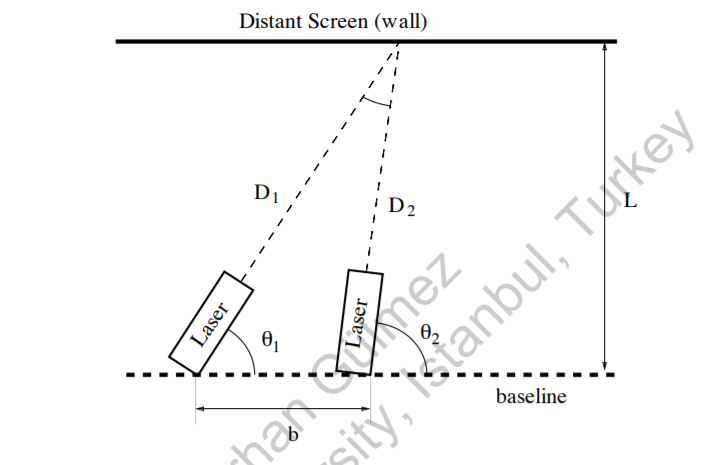
\includegraphics[scale=0.7]{triang.png}
	\end{center}
\end{figure}
\par By using the equations we have derived for $D_1$ and $D_2$ in theory part of the report we found them as
\par $D_1=111.5\pm 0.8$cm and $D_2=108.3\pm0.7$cm.
\par By finding the sines of $\theta_1=73\pm1^o$ and $\theta_2=80\pm1^o$ we can find L as
\par $L_1=106.6\pm0.8$cm and $L_2=106.6\pm0.8$cm.
\par The value we found for the length is $L=106.6\pm0.8$cm and it is 3.0$\sigma$ away from the value we have measured.\\[\baselineskip]
\textbf{\small{Finding the wavelength of the laser}}
\par From the equation:
\begin{figure}[H]
	\begin{center}
		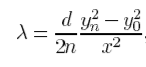
\includegraphics[scale=0.8]{lambda.png}
	\end{center}
\end{figure}
\par We have inserted our datas to the formula above and we have got 7 different $\lambda$s. Since we have done our measurements with the same apparatus, they have the same uncertainty, therefore, taking the weighted average is easy this time and we get $\lambda_{weighted}=5.5\times 10^{-5}$cm. To calculate the error of the wavelength, we use error propagation formula in the theory part of the reort and obtain $\sigma_{\lambda}=3.7\times 10^{-5}$cm.
\par Then the wavelength is  $\lambda=(5.5\pm3.7)\times 10^{-5}$cm. This is 0.22$\sigma$ away from the accepted value of the wavelength of the laser which is 633nm.
\begin{figure}[H]
	\begin{center}
		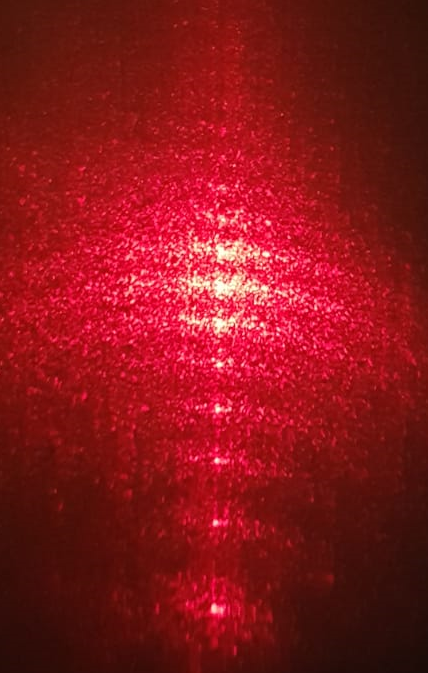
\includegraphics[scale=0.7]{2.png}
	\end{center}
\end{figure}
The photograph of diffraction pattern.\\[\baselineskip]
\textbf{\small{Finding the diameter of a hair}}
\\[\baselineskip]
\par We know n,x and $\lambda$, we used here our measured value for $\lambda$, in the minima equation $d\mathrm{sin}{\theta }_{n}=n\lambda$. Then by finding $\theta_n$ we can easily get the value of d which is diameter of hair.
\par First, we subtract our origin from the $y_n$ values to not deal with extra values. The error of each $y_n$s becomes 0.14cm.
\begin{figure}[H]
	\begin{center}
		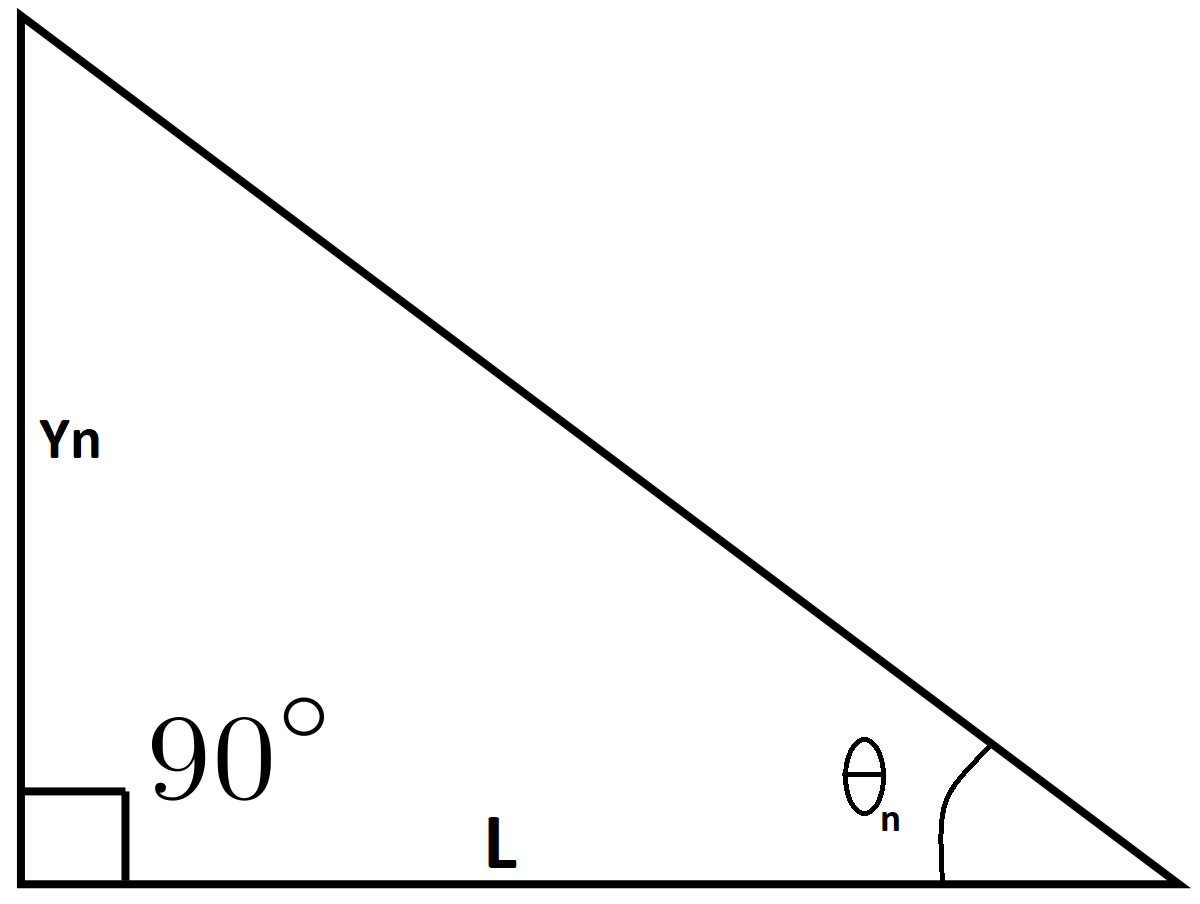
\includegraphics[scale=0.2]{tr.png}
	\end{center}
\end{figure}
\par By taking the arctan of the $y_n/x$ values, we got $\theta_n$ values. We inserted these values into the minima equation and we got 18 d values. By taking weighted average of them using the weighted average formula in the theory part of the report then we get: d=0.010cm
\par To calculate the uncertainty of d we use the error propagation formula for the minima formula then we get: $d_{error}=0.001$cm.
\par The diameter of the hair we have found is $d=0.010\pm0.001$cm.
\\[\baselineskip]
\textbf{\small{Finding the index of refraction of solid sample}}\\[\baselineskip]
\par Using the equation we have derived in theory part, we insert the d, m, $\lambda$ values to the equation:
\begin{figure}[H]
	\begin{center}
		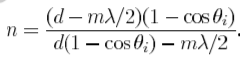
\includegraphics[scale=0.8]{in.png}
	\end{center}
\end{figure}
\par To find $\theta$, we convert the turning units to cm by dividing them with $4.00\pm0.1$ and then by using the same steps as finding the diameter of a hair part of the analysis we found $\theta$s. Now we insert our found $\theta$s to the above equation and we get many values for index of refraction. by taking the weighted average of these values we can get one value for n. Just using the formula at the theory part of the report we get $n=1.09$
\par Then by using the error propagation formula we found the error on n as 0.14.
\par The index of refraction is $n=1.09\pm0.14$.
\\[\baselineskip]\textbf{Conclusion}\\[\baselineskip]
\par We have observed some optical phenomena of lasers. For the first part of the experiment, the value we have found is 3$\sigma$ away from the value we have measured with a ruler. This is really bad value because we have wanted to measure distance more precise with laser then a ruler. Of course we have shifted the ruler a bit too much so our values coming from laser measurement can be more ''true''. But we have no way of knowing this so I don't believe our experiment is sufficient enough. We could have used more advanced equipments for measuring purposes.
\par For the second part of the experiment, our value is 0.22$\sigma$ away from the accepted value of the wavelength. This is a good value because it is very close to the accepted value. We have done this part rather well but we had problem aligning the ruler and the laser. Creating more special/advance equipment for these reasons would go a long way in reducing the time that takes to do the experiment.
\par For the third part of the experiment, our value is in the range of human hair diameter. It is hard to say many things about this value because human hair's diameter changes human to human, it is not a single value. Therefore, there might be unseen errors. For example, the hair might be a little slanted from the horizantal causing shift on the screen.
\par For the final part of the experiment, we have found the index of refraction as $n=1.09\pm0.14$. We don't know the name of the material and its index of refraction as a given value. Therefore, we couldn't make any comparision with its real value. On the other hand, we can say that we weren't very careful throught conducting the experiment. For example, seeing the fringes was really hard and even counting number of fringes passed was harder because at some point as a human we need to blink. Probably when we blinked we missed some of the fringes. Using a more powerful laser may solve these problems and also using a bit more stable and flat screen be better.
\\[\baselineskip]\textbf{References}\\[\baselineskip]
\par[1]Institute of Physics, Case study: Laser; https://www.iop.org/cs/page\_43644.html\#gref
\par[2]https://web.mit.edu/8.13/8.13c/references-fall/optics/schawlow-ajp-measuring-wavelength-of-light-with-ruler-vol33-1965.pdf
\par[3]http://labman.phys.utk.edu/phys222core/modules/m9/diffraction.htm
\par[4]Advanced Physics Experiments - Gülmez, Prof. Dr. Erhan.
\\[\baselineskip] \textbf{Appendix}\\[\baselineskip]
d
\end{document}